In the following sections the basic commands of \OCMAT\ are explained and examples are given.

\section{Initialization}
To initialize and automatically generate the \MATL\ files for a new file the initialization file has to be processed. This step has to be done only once, as long as the model (initialization file) does not change.
\begin{matlab}
function [ocStruct,datafilename]=processinitfile(initfilename,opt)(*@\index{Command!Initialization!\lstinline+processinitfile+|indexbf}@*)
%
% PROCESSINITFILE is the main file to read the initialization file
% describing the optimal control model.
%
% OCSTRUCT=PROCESSINITFILE(INITFILENAME) INITFILENAME is the name of the
% initialization file. This file has to be located in a folder on the
% MATLAB path. The name of the initialization file is given by the
% INITFILENAME and extension 'ocm'. For the structure of the initialization
% file see examples in the 'initfiles' folder. OCSTRUCT is a structure
% containing the necessary information for a further processing and
% automatic file generation.
%
% OCSTRUCT=PROCESSINITFILE(INITFILENAME,OPT) OPT is an the ocoption
% structure.
% OPT.INIT.MessageDisplay='on'/'off': turning 'on'/'off' the more detailed
%       messaging about the processing of the initialization file 
% OPT.INIT.TestConsistency='on'/'off': turning 'on'/'off' the consistency
%       test for the initialization file.
%
% [OCSTRUCT,DATAFILENAME]=PROCESSINITFILE(...) DATAFILENAME is the full
% filename, where the structure OCSTRUCT is stored. The default path and
% filename are.
% ocmat/model/usermodel/[modelname]/data/[modelname]ModelDataStructure.mat
\end{matlab}

\paragraph{Example}
To start the initialization process of model \MoM, see \cref{sec:InitializationMoM}, the initialization file \lstinline+mom.ocm+ has to be processed.
\begin{matlab}
>> [ocStruct,datafilename]=processinitfile('mom')
ocStruct = 
             modeltype: 'standardmodel'
             modelname: 'mom'
              variable: [1x1 struct]
            constraint: [1x1 struct]
             objective: [1x1 struct]
      optimizationtype: 'max'
             parameter: [1x1 struct]
           description: {'a model of moderation, simple one state model with indifference solutions'}
                   arc: [1x1 struct]
    pontryaginfunction: [1x1 struct]
                   foc: [1x1 struct]
datafilename =
\ocmat\model\usermodel\mom\data\momModelDataStructure.mat

>> opt=setocoptions('INIT','MessageDisplay','on');
>> ocStruct=processinitfile('mom',opt);
Initialization file passed the main syntax consistency test.

Initialization file passed the consistency test for the derived model structure.

The necessary conditions are derived using the symbolic toolbox version 3.2.2.
The necessary conditions are successfully derived.

\ocmat\model\usermodel\mom does not exist. Create it?  (y)/n: y
\ocmat\model\usermodel\mom\data does not exist. Create it?  (y)/n: y
Model folder(s) are successfully created:
\ocmat\model\usermodel\mom
\ocmat\model\usermodel\mom\data

\ocmat\model\usermodel\mom\data is not on MATLAB path. Add it?  (y)/n: y
Data structure 'ocStruct' is successfully stored in file:
\ocmat\model\usermodel\mom\data\momModelDataStructure.mat.
\ocmat\model\usermodel\mom is not on MATLAB path. Add it?  (y)/n: y
\end{matlab}
The instantiation of the class \lstinline+stdocmodel+ creates the main object \OCMAT\ is working with. This instance contains all information about the model and (numerical) results can be stored within this object.
\begin{matlab}
function ocObj=stdocmodel(firstarg,Result)(*@\index{Command!\lstinline+stdocmodel+|indexbf}\label{cmd:stdocmodel}@*)
%
% STDOCMODEL initializes a standard ocmodel. This object consits of two
% fields MODEL and RESULT.
%
% STDOCMODEL() an empty object is returned
%
% STDOCMODEL(OCSTRUCT) 'OCSTRUCT' is a regular model structure, as e.g.
% returned by the initialization process 
%
% STDOCMODEL(MODELNAME) the model structure is loaded from the data file
% stored in the corresponding user data folder and generated during the
% initialization process.
%
% STDOCMODEL(FILENAME) the model structure is loaded from the data file
% 'FILENAME', where 'FILENAME' is either on the MATLAB path or has to
% consist of the full path.
%
% STDOCMODEL(.,RESULT) RESULT is a structure storing results for the model.
\end{matlab}
\paragraph{Example}
\begin{matlab}
>> m=stdocmodel('mom')
Model data structure successfully loaded from data file:
F:\home\dieter\Eigene Dateien\Matlab\toolbox\numtools\ocmatnew\model\usermodel\mom\data\momModelDataStructure.mat
m =
ocmatclass: stdocmodel
    modelname : mom
    r : 1
    c : 2
		
>> m=stdocmodel([])
m =
empty stdocmodel

>> ocStruct=processinitfile('mom');
>> m=stdocmodel(ocStruct)
m =
ocmatclass: stdocmodel
    modelname : mom
    r : 1
    c : 2
\end{matlab}
The necessary files for the numerical analysis of a model can be created automatically.
\begin{matlab}
function modelfiles=makefile4ocmat(ocStruct)(*@\index{Command!Initialization!\lstinline+makefile4ocmat+|indexbf}@*)
%
% MAKEFILE4OCMAT generates the specific modelfiles from general template
% files.
%
% MODELFILES=MAKEFILE4OCMAT(OCSTRUCT) OCSTRUCT is the model structure
% generated and stored during the processing of the initialization file.
% The specific model files, e.g. the file fore the canonical system,
% Hamiltonian, etc., are build from general template files. These template
% files can be found in 'ocmat\model\standardmodel\templatefiles'. On basis
% of these template files the user can create her/his own template files.
%
% In the m-file GETMODELFILENAMES the filenames and some properties are
% defined that are then actually created. MODELFILES is a structure array
% that is returned by GETMODELFILENAMES.
% MODELFILES.NAME: basic name of a specific file (e.g. 'OptimalControl')
%           .TRANSFORMTYPE: determines if the terms are considered
%               vectorized/symbolic form
%           .FILENAME: full name of the specific file (e.g.
%               'F:\Matlab\ocmat\model\usermodel\out\momOptimalControl.m') 
\end{matlab}
\paragraph{Example}
\begin{matlab}
>> modelfiles=makefile4ocmat(ocStruct)
modelfiles = 
27x1 struct array with fields:
    name
    transformtype
    filename

>> m=stdocmodel('mom');
>> modelfiles=makefile4ocmat(m);
\end{matlab}
The newly created files are placed at an intermediate folder \lstinline+\ocmat\model\usermodel\out+. This is thought as a precautionary measure not to override already existing model files by accident. From this intermediate folder the model files can be moved to the default model folder.
\begin{matlab}
function varargout=moveocmatfiles(ocStruct,modelfiles,varargin)(*@\index{Command!Initialization!\lstinline+moveocmatfiles+|indexbf}@*)
%
% MOVEOCMATFILES moves the generated files to the model folder
%
% MOVEOCMATFILES(OCOBJ,MODELFILES) moves the files 'MODELFILES' from the
% standard output folder to the standard model folder.
%
% STATUS = MOVEOCMATFILES(OCOBJ,MODELFILES,OPT,FORCE,DIR) The resulting
% status and standard output from the operating system are returned.
\end{matlab}
\paragraph{Example}
If the model is initialized for the first time and files are created and placed at the intermediate folder the process of moving is ``quiet''.
\begin{matlab}
>> moveocmatfiles(ocStruct,modelfiles);
\end{matlab}
If files already exist in the model folder you are asked what to do.
\begin{matlab}
>> moveocmatfiles(ocStruct,modelfiles);
momArcInfo.m' already exists in \ocmat\model\usermodel\mom. Overwrite it?  y/a/(n)/q: y
momArcDiscretizationInfo.m' already exists in \ocmat\model\usermodel\mom. Overwrite it?  y/a/(n)/q: y
momCanonicalSystem.m' already exists in \ocmat\model\usermodel\mom. Overwrite it?  y/a/(n)/q: a
\end{matlab}
You can force not to ask and override
\begin{matlab}
>> moveocmatfiles(ocStruct,modelfiles,[],1);
\end{matlab}
If some file(s) named in \lstinline+modelfiles+ do not exist you receive a message
\begin{matlab}
>> moveocmatfiles(ocStruct,modelfiles);
File momCanonicalSystem.m in output folder \ocmat\model\usermodel\out does not exist.
\end{matlab}
Each instance of the class \lstinline+stdocmodel+ has a specific set of parameter values assigned. These parameter values can be retrieved or changed.
\begin{matlab}
function [parval,parvar]=parametervalue(ocObj)(*@\index{Command!stdocmodel!\lstinline+parametervalue+|indexbf}@*)
%
% PARAMETERVALUE returns the set of parameter values for the actual
% oc-model.
%
% [PARVAL,PARVAR]=PARAMETERVALUE(OCOBJ) OCOBJ is an instance of the
% stdocmodel class. The function returns the values of the parameter PARVAL
% and a cell array of strings consisting of the parameter variable names
% PARVAR.
\end{matlab}
\begin{matlab}
function ocObj=changeparametervalue(ocObj,varargin)(*@\index{Command!stdocmodel!\lstinline+changeparametervalue+|indexbf}\label{cmd:changeparametervalue}@*)
%
% CHANGEPARAMETERVALUE returns and stdocmodel with new parameters
%
% CHANGEPARAMETERVALUE(OCOBJ,PAR) returns an optimal control model with
% changed parameter values PAR. The number of parameter values PAR have to
% equal the number of parameter values of 'stdocmodel' OCOBJ. If the
% parameter values are changed the 'Result' field of the new model is
% empty. 
% 
% CHANGEPARAMETERVALUE(OCOBJ,IDX,VALUE) assigns the value VALUE to the
% parameter with  index IDX and returns the 'stdocmodel' OCOBJ with this
% changed parameter. One or more parameters can be changed, an example for
% changing one parameter would be ocObj=changeparametervalue(ocObj,1,0.05),
% for changing more parameters 
% ocObj=changeparametervalue(ocObj,[1 2 3],[0.5 1.5 4.02]). 
%
% CHANGEPARAMETERVALUE(OCOBJ,NAME,VALUE) assigns a certain value VALUE to
% the parameter with the name NAME and returns the oc model with this
% changed parameter. One or more parameters can be changed, names of
% different parameters have to be seperated by a comma e.g.
% ocObj=changeparametervalue(ocObj,'alpha,beta',[1.5 2.1]).
% or
% ocObj=changeparametervalue(ocObj,{'alpha','beta'},[1.5 2.1]).
\end{matlab}
\paragraph{Example}
\begin{matlab}
>> m=stdocmodel('fishery2D');
Model data structure successfully loaded from data file:
F:\home\dieter\Eigene Dateien\Matlab\toolbox\numtools\ocmatnew\model\usermodel\fishery2D\data\fishery2DModelDataStructure.mat
>> [par parname]=parametervalue(m)
par =
    0.0300    0.0500    1.0000    1.0000    1.0000    1.0000    1.0000         0    2.0000
parname = 
    'r'    'd'    'e'    'n'    'epsilon'    'p'    'sigma'    'ulow'    'C'
		
>> m=changeparametervalue(m,'C,d,e,n',[0.55 0.05 1.5 30])
m =
ocmatclass: stdocmodel
    modelname : fishery2D
    r : 0.03
    d : 0.05
    e : 1.5
    n : 30
    epsilon : 1
    p : 1
    sigma : 1
    ulow : 0
    C : 0.55
\end{matlab}
An easy way for the substitution of the parameter values of the current model instance in a symbolic expression.
\begin{matlab}
function s=subsparametervalue(ocObj,s)(*@\index{Command!stdocmodel!\lstinline+subsparametervalue+|indexbf}@*)
% SUBSPARAMETERVALUE substitutes the model parameters
%
% S=SUBSPARAMETERVALUE(OCOBJ,S) substitutes the parameter values of the
% optimal control model OCOBJ for the expression S, where S can be a
% character or symbolic variable.
\end{matlab}
\paragraph{Example}
\begin{matlab} 
>> m=stdocmodel('fishery2D');
>> dxdt=canonicalsystem(m,[],1,1)
dxdt =
                                                             sigma*F*(1-F/A)-1/C*F^2/(1+F^2)-ulow*F
                                                                              (n-d*A-e*A*F)*epsilon
 r*lambda1-p*ulow-lambda1*(sigma*(1-F/A)-sigma*F/A-2/C*F/(1+F^2)+2/C*F^3/(1+F^2)^2-ulow)+lambda2*e*A*epsilon
                                           r*lambda2-lambda1*sigma*F^2/A^2-lambda2*(-d-e*F)*epsilon
>> dxdt_s=subsparametervalue(m,dxdt)
dxdt_s =
                                         F*(1-F/A)-1/2*F^2/(1+F^2)
                                                      1-1/20*A-A*F
 3/100*lambda1-lambda1*(1-2*F/A-F/(1+F^2)+F^3/(1+F^2)^2)+lambda2*A
                   3/100*lambda2-lambda1*F^2/A^2-lambda2*(-1/20-F)
\end{matlab}
If a model and/or data folder for a specific \lstinline+stdocmodel+ is not on the \MATL\ path these folders can simply be added.
\begin{matlab}
function addmodelpath(modelname,force)(*@\index{Command!stdocmodel!\lstinline+addmodelpath+|indexbf}@*)
%
% ADDMODELPATH add model and data path to MATLAB search path.
%
% ADDMODELPATH(MODELNAME) MODELNAME is either a string with the name of the
% model or an OCOBJ. 
%
% ADDMODELPATH(MODELNAME,FORCE) If FORCE is 1 the model and data folder are
% added to the MATLAB path independently if the folder is already on the
% MATLAB path. If FORCE is 0 the user is asked, if the folder is not on the
% MATLAB path
\end{matlab}
\begin{matlab}
function rmmodelpath(modelname,force)(*@\index{Command!stdocmodel!\lstinline+rmmodelpath+|indexbf}@*)
%
% RMMODELPATH(MODELNAME) removes the model and data path from the MATLAB
% path. 
%
% RMMODELPATH(MODELNAME,FORCE) If FORCE is 1 the model and data folder are
% remove from the MATLAB path, otherwise (0) the user is asked if s/he
% wants to continue.
\end{matlab}
\paragraph{Example}
\begin{matlab}
>> m=stdocmodel('fishery2D');
Model data structure successfully loaded from data file:
\ocmat\model\usermodel\fishery2D\data\fishery2DModelDataStructure.mat

>> addmodelpath(m)

>> rmmodelpath(m)
Remove \ocmat\model\usermodel\fishery2D from MATLAB path?  y/(n): y
Remove \ocmat\model\usermodel\fishery2D\data from MATLAB path?  y/(n): y

>> addmodelpath(m)
\ocmat\model\usermodel\fishery2D is not on MATLAB path. Add it?  (y)/n: y
\ocmat\model\usermodel\fishery2D\data is not on MATLAB path. Add it?  (y)/n: y
\end{matlab}
During the numerical analysis you usually store the results in the instance of the analyzed \lstinline+stdocmodel+. You can save the model and its results for future work.
\begin{matlab}
function save(ocObj,varargin)(*@\index{Command!stdocmodel!\lstinline+save+|indexbf}\label{cmd:save}@*)
%
% SAVE saves an optimal control model
%
% SAVE(OCOBJ,'WORKSPACE') stores all variables from the current MATLAB
% workspace into the model specific mat-file [modelname]Workspace, located
% in the default model data folder.
%
% SAVE(OCOBJ) saves the data of an optimal control model under the standard
% data directory with the name composed of the name of the model and its
% parameter values.
%
% SAVE(OCOBJ,FORMAT) uses the format string FORMAT (see SPRINTF for
% details) for the parameter values.
%
% SAVE(OCOBJ,FORMAT,FORCE) FORCE = 1 forces to overwrite an already
% existing file. Default value is 0.
%
% SAVE(OCOBJ,FORMAT,FORCE,FN) FN provides an alternative filename.
%
% SAVE(OCOBJ,FORMAT,FORCE,[],IDX) filename is generated of the model
% name and the parameter values for the IDX'th parameter values. 
\end{matlab}
\paragraph{Example}
\begin{matlab}
>> m=stdocmodel('fishery2D');
>> save(m)
>> ocEP=calcep(m);b=isadmissible(ocEP,m,[],'UserAdmissible');ocEP(~b)=[];store(m,ocEP);
>> save(m)
Overwrite existing file from 12-Sep-2013 18:15:37 of size 1687 with new size 2252?  y/(n): y
>> filename(m)
ans =
fishery2D_r_0.03_d_0.05_e_1_n_1_epsilon_1_p_1_sigma_1_ulow_0_C_2
\end{matlab}
The user is asked if s/he wants to override the existing \lstinline+mat+-file. The file name is compounded of the model name, the parameter variables and the parameter values. The file is stored in the binary \lstinline+MAT+-file format (see \lstinline+matlab/save+).
\begin{matlab}
>> save(m,[],1)
\end{matlab}
An already existing \lstinline+mat+-file is overwritten without warning.
\begin{matlab}
>> save(m,'%1.1f',[],[1 2])
>> filename(m,'%1.1f',[1 2])
ans =
fishery2D_r_0.0_d_0.1
\end{matlab}
The file name is compounded of the model name, the first and second parameter variables and the parameter values in the format \lstinline+'%1.1f'+ (see \lstinline+matlab/fprintf+).
\begin{matlab}
>> save(m,'%1.1f',[],[1 2],'./')
\end{matlab}
The \lstinline+mat+-file is stored in the current directory \lstinline+'./'+.

Saved model instances can be reloaded. Since these files are stored as \lstinline+mat+-files you can use the \lstinline+load+ command if you know the file name. To ease the handling the \lstinline+load+ command is overloaded for \lstinline+stdocmodel+.
\begin{matlab}
function load(ocObj0,varargin)(*@\index{Command!stdocmodel!\lstinline+load+|indexbf}\label{cmd:load}@*)
%
% LOAD loads the data for oc model into the workspace
%
% LOAD(OCOBJ) loads the data for oc model into the workspace
%
% LOAD(OCOBJ,'WORKSPACE') loads data previously stored by the
% SAVE(OCOBJ,'WORKSPACE') command.
%
% LOAD(OCOBJ,FORMAT) uses the format string FORMAT (see SPRINTF for
% details) for the parameter values used for the file name generation.
%
% LOAD(OCOBJ,FORMAT,FORCE) FORCE = 1 forces to overwrite the results of
% OCOBJ by the data stored from a previous session. FORCE = 0 if a data
% file exists the user is asked if s/he wants to proceed and overwrite the
% model data.
%
% LOAD(OCOBJ,FORMAT,FORCE,FN) FN provides an alternative filename.
%
% LOAD(OCOBJ,FORMAT,FORCE,IDX) filename is generated of the model
% name and the parameter values for the IDX'th parameter values. 
%
% LOAD(OCOBJ,FORMAT,FORCE,FN,SAVEDIR) SAVEDIR provides an alternative
% folder. 
\end{matlab}
\paragraph{Example}
\begin{matlab}
>> m=stdocmodel('fishery2D');
>> m.Result
ans = 
0x0 struct array with no fields.
>> load(m)
The results in the actual model 'm' are overwritten. Proceed? y/(n) : y
>> m.Result
ans = 
    Equilibrium: {[1x1 dynprimitive]  [1x1 dynprimitive]  [1x1 dynprimitive]}
		
>> load(m,'%1.1f',[],[1 2])
The results in the actual model 'm' are overwritten. Proceed? y/(n) : y		
\end{matlab}
\begin{matlab}
function varargout=state(ocObj)(*@\index{Command!stdocmodel!\lstinline+state+|indexbf}@*)
%
% STATE returns the state values.
% 
% X=STATE(OCOBJ) OCOBJ is a stdocmodel class. X is a cell array of strings
% consisting of the state variable names. 
\end{matlab}
\begin{matlab}
function varargout=costate(ocObj)(*@\index{Command!stdocmodel!\lstinline+costate+|indexbf}@*)
%
% COSTATE returns the costate values.
% 
% L=COSTATE(OCOBJ) OCOBJ is a stdocmodel class. L is a cell array of
% strings consisting of the costate variable names. 
\end{matlab}
\begin{matlab}
function varargout=control(ocObj)(*@\index{Command!stdocmodel!\lstinline+control+|indexbf}@*)
%
% CONTROL returns the control values.
% 
% U=CONTROL(OCOBJ) OCOBJ is a stdocmodel class. U is a cell array of
% strings consisting of the terms derived from the maximum Hamiltonian
% condition (explicit control) or control variable names (implicit
% control).  
\end{matlab}
\begin{matlab}
function varargout=lagrangemultiplier(ocObj,solObj,varargin)(*@\index{Command!stdocmodel!\lstinline+lagrangemultiplier+|indexbf}@*)
%
%
% LAGRANGEMULTIPLIER returns the values of the Lagarangian multipliers.
% 
% LM=LAGRANGEMULTIPLIER(OCOBJ) OCOBJ is a stdocmodel class. LM is a cell
% array of strings consisting of the terms of the Lagarangian multiplier
% derived from the maximum Hamiltonian condition (explicit case) or the
% variable names of Lagarangian multipliers (implicit case).  
\end{matlab}
\begin{matlab}
function varargout=hamiltonian(ocObj,varargin)(*@\index{Command!stdocmodel!\lstinline+hamiltonian+|indexbf}@*)
%
% HAMILTONIAN returns the symbolic Hamiltonian or evaluated at a solution object.
% 
% H=HAMILTONIAN(OCOBJ) OCOBJ is a stdocmodel class. H is a string of the
% formally compounded (extended) Hamiltonian.
% 
% H=HAMILTONIAN(OCOBJ,[],ARCARG,1) ARCARG is the identifier for the used
% combination of active and inactive constraints. Then, H is given by the
% string expression for the maximized Hamiltonian (control variables are
% replaced by its explicit terms). The argument 1 triggers the replacement
% of the control variables (and in case of active constraints of the
% Lagrangian mutlipliers).
\end{matlab}
\begin{matlab}
function varargout=canonicalsystem(ocObj,varargin)(*@\index{Command!stdocmodel!\lstinline+canonicalsystem+|indexbf}@*)
%
% CANONICALSYSTEM returns the value of the canonical system
%
% CANONICALSYSTEM(OCOBJ) returns the symbolic expression of the canonical
% system in its general form, i.e., control variables (Lagrangian
% multipliers) are not substituted.
\end{matlab}
\paragraph{Example}
\begin{matlab}
>> addmodelpath('terrornpubop');
.\ocmat\model\usermodel\terrornpubop is not on MATLAB path. Add it?  (y)/n: y
.\ocmat\model\usermodel\terrornpubop\data is not on MATLAB path. Add it?  (y)/n: y
>> m=stdocmodel('terrornpubop');
>> state(m)
ans = 
    'T'    'P'
>> costate(m)
ans = 
    'lambda1'    'lambda2'
>> control(m)
ans =
-lambda1*eta*T^beta*P^gamma/(-1+2*lambda2*rho)
>> m=stdocmodel('fishery2D');
>> hamiltonian(m)
ans =
p*h*F-h^2+lambda1*(sigma*F*(1-F/A)-1/C*(F^2/(1+F^2))-h*F)+lambda2*((n-d*A-e*A*F)*epsilon)+lagmcc1*(h-ulow)
>> hamiltonian(m,[],0,1)
ans =
p*(1/2*p*F-1/2*lambda1*F)*F-(1/2*p*F-1/2*lambda1*F)^2+lambda1*(sigma*F*(1-F/A)-1/C*F^2/(1+F^2)-(1/2*p*F-1/2*lambda1*F)*F)+lambda2*(n-d*A-e*A*F)*epsilon
>> hamiltonian(m,[],1,1)
ans =
p*ulow*F-ulow^2+lambda1*(sigma*F*(1-F/A)-1/C*F^2/(1+F^2)-ulow*F)+lambda2*(n-d*A-e*A*F)*epsilon
>> dxdt=canonicalsystem(m)
dxdt =
                                                                   sigma*F*(1-F/A)-1/C*(F^2/(1+F^2))-h*F
                                                                                   (n-d*A-e*A*F)*epsilon
 r*lambda1-(p*h+lambda1*(sigma*(1-F/A)-sigma*F/A-2/C*F/(1+F^2)+2/C*F^3/(1+F^2)^2-h)-lambda2*e*A*epsilon)
                                              r*lambda2-(lambda1*sigma*F^2/A^2+lambda2*(-d-e*F)*epsilon)
\end{matlab}

\section{Numerical Analysis}
In the following sections the most important commands for the numerical analysis of \OCMOD\ \cref{eq:simple_simple_opt_pro} are presented. This covers particularly the calculation and handling of equilibria (instances of the \lstinline+dynprimitive+ class) and the computation of (stable) saddle-paths (instances of the \lstinline+ocasymptotic+ class) converging to an equilibrium. At this point only the \OCMat\ commands are introduced and explained. The numerical procedure is only shortly mentioned, a detailed presentation can be found in \citet{grass2012}.

\subsection{Equilibrium ('dynprimitive')}
\label{sec:EquilibriumDynprimitivecommand}

One of the first steps in the numerical analysis of an \OCPRO\ of type \cref{eq:simple_simple_opt_pro} is the search for equilibria of the canonical system. Due to the importance of equilibria these are realized as objects of the class \lstinline+dynprimitive+.\footnote{The class name is an abbreviation for ``dynamic primitives,'' where ``primitive'' is meant in the sense of ``basic.''} The implementation as a class allows an easy handling and overloading of functions.
\begin{matlab}
function ocEP=calcep(ocObj,varargin)(*@\index{Command!dynprimitive!\lstinline+calcep+|indexbf}@*)
%
% CALCEP calculates equilibria of an ocmodel.
%
% CALCEP(OCOBJ) calculates the equilibrium for the canonical system of the
% ocmodel OCOBJ using the symbolic toolbox.
%
% CALCEP(OCOBJ,X0) calculates the equilibrium numerically with starting
% values given at X0. If X0 is empty symbolic calculation is applied. For
% the numerical calculation 'FSOLVE' is used by default. 
%
% CALCEP(OCOBJ,X0,ARCARG) equilibria are calculated for the canonical
% system corresponding to arc ARCARG. If ARCARG is empty or missing the
% equilibria for every arc are computed.
%
% CALCEP(OCOBJ,X0,ARCARG,OPT) in the ocoption structure OPT options for the
% numerical solver can be provided (category OPT.EQ). In the category
% GENERAL the equation sover can be changed
% opt.GENERAL.EquationSolver='fsolve' or ...
%
% EP = CALCEP(...) the output argument EP is a cell array of 'dynprimitive'
% instances.
\end{matlab}
\begin{remark}
Keep always in mind that, whatever \lstinline+calcep+ returns
\begin{itemize}
	\item can be a numeric artifact (no equilibrium at all).
	\item need not be admissible, e.g. does not satisfy the constraints.
	\item may not be real valued.
	\item may not lie within the region of interest.
	\item etc...
\end{itemize}
\end{remark}
\paragraph{Example}
The canonical system of \MoM\ is simple enough such that the equilibria can be found using the symbolic toolbox of \MATL\ (\lstinline+sym/solve+). Anyhow, for the used parameter values two of the detected equilibria are complex valued and can therefore be omitted.
\begin{matlab}
>> m=stdocmodel('mom');
>> m=changeparametervalue(m,'r',3);
>> ocEP=calcep(m);ocEP{:}
ans =
ocmatclass: dynprimitive
modelname: mom
     0
     0
ans =
ocmatclass: dynprimitive
modelname: mom
   -0.9451
   -0.4039
ans =
ocmatclass: dynprimitive
modelname: mom
    0.9451
    0.4039
ans =
ocmatclass: dynprimitive
modelname: mom
        0 - 0.7482i
        0 - 4.6683i
ans =
ocmatclass: dynprimitive
modelname: mom
        0 + 0.7482i
        0 + 4.6683i
\end{matlab}
For models with ``highly'' nonlinear dynamics the equations of the canonical system is not or is only for specific parameter values solvable with the symbolic toolbox. In the following example equilibria can be found symbolically for the default parameter values. In fact only the fifth equilibrium is a correct solution for the equations of the canonical system. In the other cases either the points or the corresponding control values are complex valued.
\begin{matlab}
>> m=stdocmodel('terrornpubop');
>> ocEP=calcep(m);ocEP{:}
ans =
ocmatclass: dynprimitive
modelname: terrornpubop
  -0.0055 + 0.0054i
  -0.0794 + 0.0701i
  16.5753 + 3.2947i
  -2.2971 + 1.5561i
ans =
ocmatclass: dynprimitive
modelname: terrornpubop
  -0.0055 - 0.0054i
  -0.0794 - 0.0701i
  16.5753 - 3.2947i
  -2.2971 - 1.5561i
ans =
ocmatclass: dynprimitive
modelname: terrornpubop
    0.0000
    0.2072
    1.0968
   -0.0004
ans =
ocmatclass: dynprimitive
modelname: terrornpubop
    0.0000
    0.9048
    4.6738
   -0.0076
ans =
ocmatclass: dynprimitive
modelname: terrornpubop
    0.0062
    0.0996
   16.8498
   -2.3564
ans =
ocmatclass: dynprimitive
modelname: terrornpubop
    0.0000
    1.3911
    6.5273
    0.0154
\end{matlab}
For a slight change in the parameter values \lstinline+sym/solve+ cannot find a solution. In that case one has to resort to a numerical procedure.
\begin{matlab}
>> m=changeparametervalue(m,'beta,gamma',[0.49 0.99]);
>> ocEP=calcep(m);
Warning: Warning, solutions may have been lost
>> ocEP=calcep(m,[0.006 0.1 17 -2.4]');ocEP{:}
ans =
ocmatclass: dynprimitive
modelname: terrornpubop
    0.0059
    0.0938
   17.0368
   -2.4252
\end{matlab}
For models with explicit constraints the arcidentifier can be provided to calculate only those equilibria for a specific combination of active and inactive constraints.
\begin{matlab}
>> m=stdocmodel('fishery2D');
>> ocEP=calcep(m);numel(ocEP)
ans =
    17
>> ocEP=calcep(m,[],0);numel(ocEP)
ans =
    12
>> ocEP=calcep(m,[],1);numel(ocEP)
ans =
     5
\end{matlab}
As mentioned above the returned equilibria may be spurious results from numerical algorithms or do not satisfy possible constraints. Therefore, it is necessary to test the admissibility of the returned values.
\begin{matlab}
function [b adminfo]=isadmissible(dynPrim,ocObj,varargin)(*@\index{Command!dynprimitive!\lstinline+isadmissible+|indexbf}@*)
%
% ISADMISSIBLE test if equilibrium/limit set is admissible
%
% ISADMISSIBLE(OCOBJ,DYNPRIM) tests if the dynprimitive object DYNPRIM or
% cell of dynprimitives is admissible in terms of the underlying optimal
% control problem OCOBJ. If DYNPRIM is an equilibrium it is also checked if
% it satisfies the zero condition of the dynamics.
%
% ISADMISSIBLE(OCOBJ,DYNPRIM,OPT) with OPT providing the tolerance for
% admissibility.
%
% ISADMISSIBLE(OCOBJ,DYNPRIM,OPT,USERFUNC) with USERFUNC providing a
% user defined function (main function name, which is then build from the
% model name + USERFUNC)  
%
% B = ISADMISSIBLE(OCOBJ,DYNPRIMJ,OPT) if the criteria are satisfied B=1
% otherwise B=0.
%
% [B INFO]= ISADMISSIBLE(OCOBJ,DYNPRIMJ,OPT) INFO is a structure with the
% examined values. 
\end{matlab}
\paragraph{Example}
\begin{matlab}
>> [b infoStruct]=isadmissible(ocEP,m)
b =
     1     0     0     0     0     0
infoStruct = 
1x6 struct array with fields:
    ConstraintValue
    ZeroValue
    UserValue
    ImaginaryValue
		
>> infoStruct(1).ZeroValue
ans =
  1.0e-015 *
         0
   -0.0001
    0.1110
         0
>> infoStruct(1).ImaginaryValue
ans =
     0
     0
     0
     0
>> infoStruct(2).ZeroValue
ans =
  1.0e-015 *
        0          
  -0.0000 + 0.0003i
  -0.2220 - 0.2220i
        0          
>> infoStruct(2).ImaginaryValue
ans =
    0.0054
    0.0701
    3.2947
    1.5561
>> infoStruct(5).ZeroValue
ans =
   -0.0000
   -0.0000
    0.3658
    0.0000
>> infoStruct(5).ImaginaryValue
ans =
     0
     0
     0
     0
\end{matlab}
The user defined function in the \FM\ model allows to remove equilibria with negative state values. Since no state constraints are formulated equilibria with negative state values are admissible within the model specifications. However, only equilibria with nonnegative state values are of ``practical'' interest.
\begin{matlab}
>> m=stdocmodel('fishery2D');ocEP=calcep(m,[],1);
>> b=isadmissible(ocEP,m)
b =
     1     0     0     0     1
		
>> [b infoStruct]=isadmissible(ocEP,m,[],'UserAdmissible');b
b =
     1     0     0     0     0
>> infoStruct(5).UserValue
ans =
   -1.1423
   -0.9155
\end{matlab}
The calculated equilibria can be stored in the Result field of the \lstinline+stdocmodel+ instance.
\begin{matlab}
function ocObj=store(ocObj,varargin)(*@\index{Command!stdocmodel!\lstinline+store+|indexbf}\index{Command!dynprimitive!\lstinline+store+|see{stdocmodel, \lstinline+store+}}\label{cmd:store}@*)
%
% STORE results
%
% OCOBJ=STORE(OCOBJ,DYNPRIM) stores the dynprimitive object DYNPRIM in the
% results of the oc object OCOBJ (DYNPRIM can also be a cell array of
% dynprimitive objects) with field name Equilbrium.  
\end{matlab}
To retrieve equilibria from previously stored in a \lstinline+stdocmodel+.
\begin{matlab}
function ocEP = equilibrium(ocObj)(*@\index{Command!stdocmodel!\lstinline+equilibrium+|indexbf}\index{Command!dynprimitive!\lstinline+equilibrium+|see{stdocmodel, \lstinline+equilibrium+}}@*)
%
% EQUILIBRIUM returns the equilibria stored in OCOBJ
%
% OCEP=EQUILIBRIUM(OCOBJ) returns a cell arry of equilibria stored in the 
% 'Result' field 'Equilibrium' of OCOBJ.
\end{matlab}
\begin{matlab}
>> store(m,ocEP);
>> m.Result
ans = 
    Equilibrium: {[1x1 dynprimitive]  [1x1 dynprimitive]  [1x1 dynprimitive]}

>> ocEP=equilibrium(m);

>> ocEP=m.Result.Equilibrium;
\end{matlab}
A couple of commands return class or model specific information of an actual equilibrium.
\begin{matlab}
function out=arcargument(dynPrim)(*@\index{Command!dynprimitive!\lstinline+arcargument+|indexbf}@*)
%
% ARCARGUMENT returns the identfier for the underlying combination of
% active and inactive constraints.
%
% ARCARG=ARCARGUMENT(DYNPRIM) DYNPRIM is a member of the class
% 'dynprimitive'. The returned argument ARCARG is the identifier specified
% within an OCMat model for a specific combination of active (binding) and
% inactive (non-binding) constraints.
\end{matlab}
\begin{matlab}
function out=dependentvar(dynPrim)(*@\index{Command!dynprimitive!\lstinline+dependentvar+|indexbf}@*)
%
% DEPENDENTVAR returns the point(s) of the dynprimitive object.
%
% P=DEPENDENTVAR(DYNPRIM) DYNPRIM is a member of the class
% 'dynprimitive', these can be interpreted either as a geometric object,
% point(s) in the phase space, or a time trajectory. The constant function
% in the case of an equilibrium, a periodic function in the case of a limit
% cycle. From the latter interpretation DEPENDENTVAR returns the (time)
% depending point(s) P of the object.
\end{matlab}
\begin{matlab}
function realdynPrim=real(dynPrim)(*@\index{Command!dynprimitive!\lstinline+real+|indexbf}@*)
%
% REAL returns the real valued object.
%
% RDYNPRIM = REAL(DYNPRIM) returns a dynprimitive object RDYNPRIM, with only 
% the real parts, as well for the dynVar field as the linearization field,
% of the dynprimitive DYNPRIM.
\end{matlab}
\begin{matlab}
function varargout=imag(dynPrim)(*@\index{Command!dynprimitive!\lstinline+imag+|indexbf}@*)
%
% IMAG returns a dynprimitive object consisting of the imaginary parts.
%
% IDYNPRIM = IMAG(DYNPRIM) returns a dynprimitive object RDYNPRIM, with only 
% the imaginary parts, as well for the dynVar field as the linearization field,
% of the dynprimitive DYNPRIM.
\end{matlab}
It happens that a returned equilibrium has spurious imaginary parts being an artifact from the numerical procedure. The command \lstinline+remspuriousimag+ tests if the imaginary parts exceed some given tolerance and returns the real valued object otherwise.
\begin{matlab}
function realdynPrim=remspuriousimag(dynPrim,opt)(*@\index{Command!dynprimitive!\lstinline+remspuriousimag+|indexbf}@*)
%
% REMSPURIOUSIMAG removes spurious imaginary part.
%
% RDYNPRIM = REMSPURIOUSIMAG(DYNPRIM) returns a dynprimitive object
% RDYNPRIM, with only  the real parts, as well for the dynVar field as the
% linearization field, of the dynprimitive DYNPRIM.
\end{matlab}
\paragraph{Example} When should \lstinline+remspuriousimag+ be applied? 
\begin{matlab}
>> m=stdocmodel('terrornpubop');
>> ocEP=calcep(m,[0.1839 0.2400 0.4173 0.0497]');ocEP{:}
ans =
ocmatclass: dynprimitive
modelname: terrornpubop
   0.0062 - 0.0000i
   0.0996 + 0.0000i
  16.8498 - 0.0000i
  -2.3564 - 0.0000i
>> imag(ocEP{1})
ans =
  1.0e-012 *
   -0.0001
    0.0011
   -0.1286
   -0.0189
\end{matlab}
A numerical calculation of the equilibrium yields a result with very small imaginary part. We expect the imaginary part to be a numerical artifact.
\begin{matlab}
>> opt=setocoptions('GENERAL','ImaginaryTolerance',1e-11);
>> dynPrimR=remspuriousimag(ocEP{1},opt)
dynPrimR =
ocmatclass: dynprimitive
modelname: terrornpubop
    0.0062
    0.0996
   16.8498
   -2.3564
>> ocEP=calcep(m,dynPrimR.y);ocEP{:}
ans =
ocmatclass: dynprimitive
modelname: terrornpubop
    0.0062
    0.0996
   16.8498
   -2.3564
\end{matlab}
To assure that the imaginary parts are only removed if the values are ``very'' small, the user can provide a tolerance \lstinline+ImaginaryTolerance+. Next we check whether this real valued dynprimitive is an admissible equilibrium. Therefore, the numerical calculation is repeated with the real valued point as initial guess, which yields the expected result.

To determine the eigenvalues and eigenvectors of the Jacobian corresponding to an equilibrium the native \MATL\ \lstinline+eig+-function is overloaded for the class \lstinline+dynprimitive+.
\begin{matlab}
function varargout=eig(dynPrim,varargin)(*@\index{Command!dynprimitive!\lstinline+eig+|indexbf}@*)
%
% EIG find eigenvalues and eigenvectors.
%
% D = EIG(DYNPRIM) returns the eigenvalues for the Jacobian/Monodromy
% matrix of the dynprimitve object DYNPRIM.    
%
% [D,V] = EIG(DYNPRIM) produces matrices of eigenvalues (D) and eigenvectors
% (V) (for more information help eig).  
\end{matlab}
\paragraph{Example}
\begin{matlab}
>> m=stdocmodel('terrornpubop');
>> ocEP=calcep(m,[0.006 0.1 17 -2.4]');
>> eig(ocEP{1})
ans =
  -0.0013 + 0.0466i
  -0.0013 - 0.0466i
   0.0413 + 0.0466i
   0.0413 - 0.0466i
	
>> [eigvec eigval]=eig(ocEP{1})
eigvec =
  -0.0007 - 0.0001i  -0.0007 + 0.0001i  -0.0002 + 0.0001i  -0.0002 - 0.0001i
  -0.0019 + 0.0033i  -0.0019 - 0.0033i  -0.0009 + 0.0027i  -0.0009 - 0.0027i
   0.9996             0.9996             0.9901             0.9901          
   0.0259 - 0.0140i   0.0259 + 0.0140i  -0.0010 - 0.1406i  -0.0010 + 0.1406i
eigval =
  -0.0013 + 0.0466i        0                  0                  0          
        0            -0.0013 - 0.0466i        0                  0          
        0                  0             0.0413 + 0.0466i        0          
        0                  0                  0             0.0413 - 0.0466i
\end{matlab}
The eigenvalues determine the behavior of the trajectories in the neighborhood of an equilibrium. If the Jacobian is non-singular the dimension of the (un)stable manifold is totally determined by the positive/negative real part of the eigenvalues. An equilibrium with positive and negative real part of the eigenvalues is called a saddle point.
\begin{matlab}
function [b,dim]=issaddle(varargin)(*@\index{Command!dynprimitive!\lstinline+issaddle+|indexbf}@*)
%
% ISSADDLE true if limit set is of saddle type
%
% B = ISSADDLE(DYNPRIM) the input argument DYNPRIM is a dynprimitve object,
% 'equilibrium' or 'limitcycle'. B is 1 if DYNPRIM is of saddle type, for
% an equilibrium at least one eigenvalue has to be negative. For a limit
% cycle the absolute value at least of one eigenvalue has to be smaller
% than one.
%
% [B DIM] = ISSADDLE(DYNPRIM) DIM returns the number of of "stable"
% eigenvalues
%
% [B DIM] = ISSADDLE(DYNPRIM,OPT) with OPT the tolerance for a zero
% eigenvalue can be provided:
%   opt=setocoptions('OC','ZeroEigenValueTolerance',tol);
%
% [B DIM] = ISSADDLE(DYNPRIM1,...,DYNPRIMN) B is a vector of 0 and 1
% depending if the dynprimitve objects DYNPRIM1,...,DYNPRIMN are of saddle
% type. DIM is a vector containing the number of "stable" eigenvlaues for
% each of the dynprimitve objects.
%
% [B DIM] = ISSADDLE(DYNPRIM1,...,DYNPRIMN,OPT)
\end{matlab}
\paragraph{Example}
\begin{matlab}
>> m=stdocmodel('fishery2D');
>> m=changeparametervalue(m,'C,d,e,n',[0.55 0.05 1.5 30]);
>> ocEP=calcep(m);b=isadmissible(ocEP,m,[],'UserAdmissible');ocEP(~b)=[];
>> [b dim]=issaddle(ocEP{:})
b =
     1     1     1     1     1
dim =
     2     2     1     2     2
\end{matlab}
The so far presented properties are inherent to a \lstinline+dynprimitive+ object, independently from the underlying \OCMOD, e.g., the stability, determined by the eigenvalues. The next set of commands need information from the specific model, e.g., the value of the states, costates, controls, etc..
\begin{matlab}
function x=state(ocObj,dynPrim)(*@\index{Command!dynprimitive!\lstinline+state+|indexbf}@*)
%
% STATE returns the state values.
% 
% X=STATE(OCOBJ,DYNPRIM) If DYNPRIM is empty the output is the same as for
% STATE(OCOBJ). Otherwise the state values of the dynprimitive object
% DYNPRIM are returned.  
\end{matlab}
\begin{matlab}
function l=costate(ocObj,dynPrim)(*@\index{Command!dynprimitive!\lstinline+costate+|indexbf}@*)
%
% COSTATE returns the costate values.
% 
% L=COSTATE(OCOBJ,DYNPRIM) If DYNPRIM is empty the output is the same as
% for COSTATE(OCOBJ). Otherwise the costate of the dynprimitive object
% DYNPRIM values are returned.  
\end{matlab}
\begin{matlab}
function u=control(ocObj,dynPrim)(*@\index{Command!dynprimitive!\lstinline+control+|indexbf}@*)
%
% CONTROL returns the control values.
% 
% U=CONTROL(OCOBJ,DYNPRIM) If DYNPRIM is empty the output is the same as
% for CONTROL(OCOBJ). Otherwise the control values of the dynprimitive
% object DYNPRIM are returned. 
\end{matlab}
\begin{matlab}
function lm=lagrangemultiplier(ocObj,dynPrim)(*@\index{Command!dynprimitive!\lstinline+lagrangemultiplier+|indexbf}@*)
%
% LAGRANGEMULTIPLIER returns the values of the Lagarangian multipliers.
% 
% LM=LAGRANGEMULTIPLIER(OCOBJ,SOLOBJ)(OCOBJ,DYNPRIM) If DYNPRIM is empty
% the output is the same as for LAGRANGEMULTIPLIER(OCOBJ). Otherwise the
% values of the Lagarangian multipliers of the dynprimitive object DYNPRIM
% are returned.  
\end{matlab}
\begin{matlab}
function H=hamiltonian(ocObj,dynPrim)(*@\index{Command!dynprimitive!\lstinline+hamiltonian+|indexbf}@*)
%
% HAMILTONIAN returns the Hamiltonian value.
% 
% H=HAMILTONIAN(OCOBJ,DYNPRIM) If DYNPRIM is empty the
% autput is the same as for HAMILTONIAN(OCOBJ). Otherwise the Hamiltonian
% evaluated at the dynprimitive object DYNPRIM is returned.
\end{matlab}
\begin{matlab}
function J=jacobian(ocObj,dynPrim)(*@\index{Command!dynprimitive!\lstinline+jacobian+|indexbf}@*)
%
% JACOBIAN returns the Jacobian matrix.
% 
% J=JACOBIAN(OCOBJ,DYNPRIM) If DYNPRIM is empty the output is the same as
% for JACOBIAN(OCOBJ). Otherwise the Jacobian evaluated at the dynprimitive
% object DYNPRIM is returned.  
\end{matlab}
\begin{matlab}
function d=canonicalsystem(ocObj,dynPrim)(*@\index{Command!dynprimitive!\lstinline+canonicalsystem+|indexbf}@*)
%
% CANONICALSYSTEM returns the value of the canonical system
%
% D=CANONICALSYSTEM(OCOBJ,DYNPRIM) If DYNPRIM is empty the output is the
% same as for CANONICALSYSTEM(OCOBJ). Otherwise the value of the canonical
% system evaluated at the dynprimitive object DYNPRIM is returned. 
\end{matlab}
\paragraph{Example}
\begin{matlab}
>> m=stdocmodel('fishery2D');
>> load(m)
The results in the actual model 'm' are overwritten. Proceed? y/(n) : y
>> ocEP=equilibrium(m);
>> state(m,ocEP{2})
ans =
    0.6870
    1.3568
>> costate(m,ocEP{2})
ans =
    0.2424
    0.0810
>> control(m,ocEP{2})
ans =
    0.2603
>> hamiltonian(m,ocEP{2})
ans =
    0.1111
>> jacobian(m,ocEP{2})
ans =
   -0.8503    0.2564    0.2360         0
   -1.3568   -0.7370         0         0
    0.0387   -0.0999    0.8803    1.3568
   -0.0999    0.0916   -0.2564    0.7670

>> m=stdocmodel('fishery2D');
>> ocEP=calcep(m,[],1);ocEP{4}
ans =
ocmatclass: dynprimitive
modelname: fishery2D
    0.8434
    1.1193
         0
         0
>> lagrangemultiplier(m,ocEP{4})
ans =
   -0.8434
\end{matlab}


\subsection{Saddle-Path ('ocasymptotic')}
\label{sec:saddlepathocasymptoticcommand}
For the calculation of a saddle-path a \BVP\ embedded into a continuation process is solved \citep[cf.~][]{grass2012}. Before the continuation is started the problem has to be initialized.
\begin{matlab}
function sol=initocmat_AE_EP(ocObj,ocEP,contcoordinate,targetvalue,opt,varargin)(*@\index{Command!continuation!\lstinline+initocmat_AE_EP+|indexbf}@*)
%
% INITOCMAT_AE_EP initialization for asymptotic extremal calculation
%
% SOL=INITOCMAT_AE_EP(OCOBJ,OCEP,CONTCOORDINATE,TARGETVALUE) a stable
% saddle path calculation is initialized. 
% OCOBJ          ... corresponding optimal control model
% OCEP           ... equilibrium point (dynprimitive) (hat-x) with (local)
%                    stable manifold of dimension k 
% CONTCOORDINATE ... coordinates i_1,...,i_k of the continuation variable
%                    (usually state coordinate(s) in optimal control
%                    problems)  
% TARGETVALUE    ... determines direction of the continuation (x_j^0,
%                    j=i_1,...,i_k) 
%
% The output argument SOL is a solution structure for a BVP with the
% standard fields 'x', 'y', 'parameters' (MATLAB syntax for BVPs).
% The (important) OCMat specific fields 
%   arcinterval ... truncation of the time interval
%   arcarg      ... arc identifier for a specific combination of active and
%                   inactive constraints.
% are provided as well.
%
% During the initialization two global variables OCMATCONT and OCMATAE are
% initialized. The first variable contains general information for the
% continuation process. The second variable contains problem specific
% information.
%
% SHORT EXPLANATION OF THE MATHEMATICAL BACKGROUND
%
% The underlying mathematical problem formulation is to find a trajectory
% (time path) x(t)=(x_1(t),...,x_N(t)) with initial condition x_j(0)=x_j^0,
% j=i_1,...,i_k and lim_{t\to\infty}x(t)=hat-x (convergence to the
% equilibrium). 
%
% The problem is solved using a continuation algorithm, where the
% continuation is done for the initial condition
%   x_j(0)=x_j^0, j=i_1,...,i_k
% and the continuation parameter 'mu' is defined as
%   x_j(0)=x_j^0*mu+(1-mu)*hat-x_j, j=i_1,...,i_k.
% Thus, for mu=0 we have
%   x_j(0)=hat-x_j, j=i_1,...,i_k
% and for mu=1
%   x_j(0)=x_j^0
% The end condition, convergence to the equilibrium, is reformulated in a
% way that allows a numerical treatment. The default way is the truncation
% of the infinite time to a finite time 'T' and the condtion that the end
% point x(T) ends on the linearized stable manifold (stable eigenspace).
%
% This means that at the start of the continuation the equilibrium path
% (constant solution at the equilibrium) trivially satisfies the initial
% and end condition. Therefore, with the provision of the equilibrium the
% initial solution is given as well. In that sense the OCEP argument
% performs two tasks. The searched for solution converges to OCEP and OCEP
% is the initial solution (mu=0) of the continuation process.
%
% The denomination as TARGETVALUE maybe misleading but from the
% continuation point of view it denotes the target. From the problem
% perspective it denotes the initial state values of the searched for
% solution. 
% 
% SOL=INITOCMAT_AE_EP(OCOBJ,OCEP,CONTCOORDINATE,TARGETVALUE,OPT) with the
% option structure OPT the threshold 'ZeroDeviationTolerance' and initial
% number of discretization points 'TrivialArcMeshNum', for the equilibrium
% solution can be changed. 
%   ZeroDeviationTolerance ... provides the tolerance to classify an 
%                              eigenvalue numerically as zero.
%   TrivialArcMeshNum      ... provides the number of points for the
%                              constant solution at the equilbrium. 
%
% SOL=INITOCMAT_AE_EP(...,'TruncationTime',T) the truncation of the
% infinite time horizon to the finite time T 
% 
% SOL=INITOCMAT_AE_EP(...,'PathType',p)
%   p='s' (default) stable saddle-path calculation
%   p='u' unstable saddle-path calculation
\end{matlab}
\begin{matlab}
function sol=initocmat_AE_AE(ocObj,ocAsym,contcoordinate,targetvalue,opt)(*@\index{Command!continuation!\lstinline+initocmat_AE_AE+|indexbf}@*)
%
% INITOCMAT_AE_AE initialization for asymptotic extremal calculation
%
% SOL=INITOCMAT_AE_AE(OCOBJ,OCASYM,CONTCOORDINATE,TARGETVALUE) the
% continuation process is initialized (started) at a solution OCASYM
% (instance of the ocasymptotic class) that (usually) has been calculated
% during a previous continuation. Therefore, neither the 'TruncationTime' ,
% nor the 'PathType' (see INITOCMAT_AE_EP) can be provided. This
% information is taken from the OCASYM object. 
%
% For a more detailed discussion see INITOCMAT_AE_EP
%
\end{matlab}
After the initialization the continuation process can be started.
\begin{matlab}
function sout=bvpcont(varargin)(*@\index{Command!continuation!\lstinline+bvpcont+|indexbf}@*)
%
% BVPCONT main OCMat continuation file for BVPs
%
% BVPCONT(PROBLEMTYPE,INITSOL) argument PROBLEMTYPE is a string
% characterizing the type of problem to be solved:
%   'extremal2ep'   ... saddle-path of an equilibrium, continuing along the
%                       initial point
%   'extremalp2ep'  ... saddle-path of an equilibrium, continuing along a
%                       parameter value
%   'extremalt2ep'  ... saddle-path of an equilibrium, continuing the
%                       truncation time
%   'indifferencesolution'  ... continuation of an indifference threshold
%                       (Skiba point)
%   'limitextremal' ... continuation of a limitpoint solution
%
% INITSOL is an initial function structure to start the continuation,
% returned by an initialization function, e.g. initocmat_AE_EP,
% initocmat_AE_IS (see OCMat manual)
%
% BVPCONT(PROBLEMTYPE,INITSOL,INITTANGENT) INITTANGENT is an initial
% tangent, usually this argument is empty.  
%
% BVPCONT(PROBLEMTYPE,INITSOL,INITTANGENT,OPT) the option structure OPT provides a
% multitude of settings for the continuation process and BVP solver (see
% OCMat manual). 
%
% SOUT=BVPCONT(...) the structure array consists at least of two elements
% from the intial and last step of the continuation.
\end{matlab}
If the option \lstinline+opt.OCCONTARG.SaveIntermediate='on'+ (default value) the solution from the continuation process are written into a \lstinline+mat+ and can be saved into the \lstinline+Result+ field of the \lstinline+stdocmodel+ object.
\begin{matlab}
function varargout=store(ocObj,varargin)(*@\index{Command!continuation!\lstinline+store+|indexbf}@*)
%
% STORE results of continuation process
%
% STORE(OCOBJ,PROBLEMTYPE) store results of continuation process
% given by PROBLEMTYPE:
%   'extremal2ep'   ... saddle-path of an equilibrium, continuing along the
%                       initial point
%   'extremalp2ep'  ... saddle-path of an equilibrium, continuing along a
%                       parameter value
%   'extremalt2ep'  ... saddle-path of an equilibrium, continuing the
%                       truncation time
%   'indifferencesolution'  ... continuation of an indifference threshold
%                       (Skiba point)
%   'limitextremal' ... continuation of a limitpoint solution
%
% STORE(OCOBJ,OCELEMENT) stores the object OCELEMENT in the Result field of
% the stdocmodel object OCOBJ. 
% Possible classes for OCELEMENT are
%        dynprimitive: equilibrium or limit cycle
%        ocasymptotic: asymptotic solutions
%        cell array of 'dynprimitives' or 'ocasymptotics'
%
% The default names of the Result field are
%       Result.Equilibrium: for a dynprimitive being an equilibrium
%       Result.LimitCycle: for a dynprimitive being a limit cycle
%       Result.ExtremalSolution: for an ocasymptotic
%       Result.Continuation: for the result of a continuation process
% If no output argument is specified it is written into the object OCOBJ.
%
% OCOBJN=STORE(...) the result is returned to the new stdocmodel instance
% OCOBJN 
\end{matlab}
To remove results from an \lstinline+stdocmodel+ object.
\begin{matlab}
function varargout=delete(ocObj,varargin)(*@\index{Command!continuation!\lstinline+delete+|indexbf}@*)
%
% DELETE deletes specific results stored in OCOBJ.
%
% DELETE(OCOBJ,FIELDNAME,INDEX) deletes the results stored under FIELDNAME
% in the Result filed of OCOBJ. INDEX is an array specifying the index of
% the results to be deleted. 
%
% DELETE(OCOBJ,FIELDNAME1,INDEX1,FIELDNAME2,INDEX2, ...) 
%
% OCOBJN=DELETE(...) the result is returned to the new stdocmodel instance
% OCOBJN 
\end{matlab}
\paragraph{Example}
\begin{matlab}
>> m=stdocmodel('mom');ocEP=calcep(m);b=isadmissible(ocEP,m);ocEP(~b)=[];store(m,ocEP);
>> sol=initocmat_AE_EP(m,ocEP{1},1,0.5);
>> c=bvpcont('extremal2ep',sol);
>> store(m,'extremal2ep');
first solution found
tangent vector to first solution found

 Continuation step No.: 1
 stepwidth: 0.01
 Newton Iterations: 1
 Mesh size: 37
 Continuation parameter: 0.00314377

 Continuation step No.: 300
 stepwidth: 0.1
 Newton Iterations: 1
 Mesh size: 134
 Continuation parameter: 0.919401
>> store(m,'extremal2ep');
>> opt=setocoptions('OCCONTARG','Backward',1,'TotalRelativeDistance',-1);
>> sol=initocmat_AE_EP(m,ocEP{1},1,0.3);
>> c=bvpcont('extremal2ep',sol,[],opt);
first solution found
tangent vector to first solution found

 Continuation step No.: 1
 stepwidth: 0.01
 Newton Iterations: 1
 Mesh size: 36
 Continuation parameter: -0.00483221


 Continuation step No.: 38
 stepwidth: 0.1
 Newton Iterations: 1
 Mesh size: 54
 Continuation parameter: -1.00676

 Target value hit.
 label=HTV
 Continuation parameter=-1
>> store(m,'extremal2ep');
>> m.Result
ans = 
     Equilibrium: {[1x1 dynprimitive]  [1x1 dynprimitive]  [1x1 dynprimitive]  [1x1 dynprimitive]  [1x1 dynprimitive]}
    Continuation: {[1x1 struct]  [1x1 struct]}
>> delete(m,'Continuation',2,'Equilibrium',[4 5]);m.Result
ans = 
     Equilibrium: {[1x1 dynprimitive]  [1x1 dynprimitive]  [1x1 dynprimitive]}
    Continuation: {[1x1 struct]}
\end{matlab}
During the continuation process the evolution of the solution is plotted into a figure window. This helps the user to ``visually'' control the output of the continuation. Additionally, basic information is displayed in the command window.
\begin{description}
	\item[stepwidth:] Step width of the continuation step.
	\item[Newton Iterations:] The number of Newton steps during the continuation step.
	\item[Mesh size:] The mesh size of the \BVP\ solution.
	\item[Continuation parameter:] Value of the continuation parameter, $1$ denotes the searched for solution.
\end{description}
In our example the continuation stops at step 300 (default maximum number of continuation steps), with a step width 0.1 (default maximum step width). The continuation parameter is smaller than $1$. Thus, a solution with $x(0)=0.5$, as stated in the initialization step, has not been reached. The reason for that can be seen in \cref{fig:basicmomcontsol}. The stable path spirals out from an unstable equilibrium and no saddle-path, starting at $x(0)=0.5$ and converging to the equilibrium at the origin exists (see also \cref{sec:numanalysis_detindthr}).

The dialog box 'UserStop', \cref{fig:userstop}, provides a possibility to interrupt the continuation process without using the often cumbersome \lstinline+Ctrl-C+ method. 
\begin{figure}
\centering
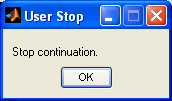
\includegraphics[scale=\scalefactor]{./fig/UserStop}
\label{fig:userstop}
\caption{Dialog box to interrupt a continuation process.}
\end{figure}
\begin{figure}
\centering
\includegraphics[scale=\scalefactor]{./fig/BasicMoMContinuationPath}
\label{fig:basicmomcontsol}
\caption{The stable saddle path of the equilibrium at the origin (green) spirals out from an unstable node (blue).}
\end{figure}

An important aspect of the calculation of stable-paths in \OCMAT\ is the possibility to handle constraints that become active on parts of the trajectory. First of all this means that possible violations of constraints have to be detected during the continuation. Secondly it is necessary to use the information about constraint violations to adapt the underlying \BVP\ and solution to restart the continuation process taking the active constraints into account.
\begin{matlab}
function solp=partialarc(sol,partarccoord)(*@\index{Command!continuation!\lstinline+partialarc+|indexbf}@*)
%
% PARTIALARC returns a part of a trajectory
%
% PARTIALARC(SOL,PARTARCCOORD) the arc of the solution structure SOl is
% returned for the indices specified by PARTARCCOORD.
%
% SOLP=PARTIALARC(SOL,PARTARCCOORD) SOLP is a solution structure, with
% adapted fields 'x', 'y', 'arcarg', 'arcinterval', 'arcposition'.
\end{matlab}
\begin{matlab}
function sol=addarc(sol,arc,iposition)(*@\index{Command!continuation!\lstinline+addarc+|indexbf}@*)
%
% ADDARC fit an arc into a solution
%
% ADDARC(SOL,ARC) the input arguments SOL and ARC are OCMat solution
% structures. ARC is placed as a new arc in front of SOL.
\end{matlab}
\paragraph{Example}
\begin{matlab}
>> m=stdocmodel('fishery2D');
>> ocEP=calcep(m);b=isadmissible(ocEP,m,[],'UserAdmissible');ocEP(~b)=[];store(m,ocEP);
>> opt=setocoptions('OCCONTARG','MaxStepWidth',1);
>> sol=initocmat_AE_EP(m,ocEP{2},1:2,[0.01 0.1],opt);
>> c=bvpcont('extremal2ep',sol,[],opt);
first solution found
tangent vector to first solution found

 Continuation step No.: 1
 stepwidth: 0.01
 Newton Iterations: 1
 Mesh size: 42
 Continuation parameter: 0.00567166

 Continuation step No.: 21
 stepwidth: 1
 Newton Iterations: 1
 Mesh size: 120
 Continuation parameter: 0.902635
 
Non admissible solution detected, reduce stepwidth.

 Continuation step No.: 22
 stepwidth: 0.5
 Newton Iterations: 1
 Mesh size: 131
 Continuation parameter: 0.915318

Non admissible solution detected, reduce stepwidth.
Current step size too small (point 29)

 Continuation step No.: 29
 stepwidth: 1e-005
 Newton Iterations: 1
 Mesh size: 131
 Continuation parameter: 0.915442

>> store(m,'extremal2ep');ocAsym=extremalsolution(m);

>> trj=partialarc(ocAsym{1},[1 1]);trj.arcarg=1;
>> ocAsymN=addarc(ocAsym{1},trj);

>> sol=initocmat_AE_AE(m,ocAsymN,1:2,[0.01 0.1],opt);
>> c=bvpcont('extremal2ep',sol,[],opt);
\end{matlab}

\subsection{Indifference Threshold}
The phenomenon that the optimal solution may not be unique is a well known phenomenon. In the large majority of cases the calculation and detection of these solutions needs to be done numerically. One of the strengths of \OCMAT\ is exactly this task, which in general (for models with at least two states) consists of two basic steps.
\begin{enumerate}
	\item The detection of an indifference threshold.
	\item The continuation of the detected indifference threshold, yielding a curve, surface, ....
\end{enumerate}
These basic steps are reflected in the actual implementation. For the detection of an indifference threshold \OCMAT\ provides the function \lstinline+findindifferencepoint+.
\begin{matlab}
function [indiffpt o]=findindifferencepoint(ocObj,sliceman1,sliceman2,varargin)(*@\index{Command!stdocmodel!\lstinline+findindifferencepoint+|indexbf}@*)
%
% FINDINDIFFERENCEPOINT find indifference threshold.
%
% FINDINDIFFERENCEPOINT(OCOBJ,IDX1,IDX2) IDX1 and IDX2 are the indices of
% continuation results stored in OCOBJ. To detect an indifference threshold
% the Hamiltonian is evaluated at the initial points of the continuation
% process (slice manifold) and intersected. The slice manifold is only
% considered from the first point to the point where it bends back, if it
% bends back at all.
%
% FINDINDIFFERENCEPOINT(OCOBJ,SLMF1,SLMF2) SLMF1 and SLMF2 are slice
% manifolds.
%
% FINDINDIFFERENCEPOINT(OCOBJ,IDX1,IDX2,OPT) 
%   OPT.GENERAL.AdmissibleTolerance defines the tolerance for the
%           collinearity test of the slice manifolds.  
%   OPT.OCCONTARG.PlotCont='on'/'off' if set 'on' the result is shown
%           graphically
%
% FINDINDIFFERENCEPOINT(OCOBJ,IDX1,IDX2,OPT,SPEC1,SPEC2) the argument
%       SPEC1= ''/'r': if set to 'r' the slice manifold is considered in
%               reverse order. This argument is useful if the threshold
%               point separates two solutions converging to the same limit
%               set. In that case it suffices to compute one slice manifold
%               (with at least two limit points) IDX and call
%               FINDINDIFFERENCEPOINT(OCOBJ,IDX,IDX,[],'r')
%
% INDIFFPT=FINDINDIFFERENCEPOINT(...) if the Hamiltonian functions
% intersect the (state) values of the intersection point INDIFFPT is
% returned otherwise it is empty.
%
% [INDIFFPT O]=FINDINDIFFERENCEPOINT(...) O is the corresponding obective
% value or empty.
\end{matlab}
This solution is used to initialize an indifference threshold continuation.
\begin{matlab}
function sol=initocmat_AE_IS(ocObj,ocMP,targetcoordinate,targetvalue,opt,fixedcoordinate,varargin)(*@\index{Command!stdocmodel!\lstinline+initocmat_AE_IS+|indexbf}@*)
%
% INITOCMAT_AE_IS initialization for the continuation of an indifference
% threshold
%
% SOL=INITOCMAT_AE_IS(OCOBJ,OCMP,TARGETCOORDINATE,TARGETVALUE) the
% continuation of an indifference threshold in the state space is
% initialized.    
% OCOBJ          ... corresponding optimal control model
% OCMP           ... two cell array of ocasymptotics, for the different
%                    solution paths or an instance of an ocmultipath
%                    object. 
% TARGETCOORDINATE ... the continuation is done along the n-1 coordinates
%                   (n number of states) 
% TARGETVALUE    ... The value of the target vector for the n-1
%                   coordinates.
%
% The output argument SOL is a solution structure for a BVP with the
% standard fields 'x', 'y', 'parameters' (MATLAB syntax for BVPs).
% The (important) OCMat specific fields 
%   arcinterval ... truncation of the time interval
%   arcarg      ... arc identifier for a specific combination of active and
%                   inactive constraints.
% are provided as well.
%
% During the initialization two global variables OCMATCONT and OCMATINDIF
% are initialized. The first variable contains general information for the
% continuation process. The second variable contains problem specific
% information.
%
% SOL=INITOCMAT_AE_IS(OCOBJ,OCMP,TARGETCOORDINATE,TARGETVALUE,OPT)
\end{matlab}
\paragraph{Example}
The following example is explained more detailed in \cref{sec:initandnumanacrm}.
\begin{matlab}
>> m=stdocmodel('harvest3D');
>> m=changeparametervalue(m,'r,l,s,w',[0.1 1 0.325 0]);
>> ocEP=calcep(m);b=isadmissible(ocEP,m,[],'UserAdmissible');ocEP(~b)=[];(*@\index{Command!stdocmodel!calcep}\index{Command!dynprimitive!isadmissible}@*)
>> [b dim]=issaddle(ocEP{:});ocEP(~b)=[];store(m,ocEP);(*@\index{Command!dynprimitive!issaddle}@*)
>> opt=setocoptions('OCCONTARG','MaxStepWidth',1,'GENERAL','BVPMethod','bvp6c');
>> opt=setocoptions(opt,'OCCONTARG','MaxContinuationSteps',100);
>> sol=initocmat_AE_EP(m,ocEP{1},1:3,ocEP{2}.y(1:3),opt,'TruncationTime',1000);
>> c=bvpcont('extremal2ep',sol,[],opt);
>> store(m,'extremal2ep');
>> opt=setocoptions(opt,'OCCONTARG','MaxStepWidth',50);
>> sol=initocmat_AE_EP(m,ocEP{2},1:3,ocEP{1}.y(1:3),opt,'TruncationTime',1000);
>> c=bvpcont('extremal2ep',sol,[],opt);
>> store(m,'extremal2ep');
>> ocAsym=extremalsolution(m);
>> trj=partialarc(ocAsym{2},[1 1]);trj.arcarg=1;
>> ocAsymN=addarc(ocAsym{2},trj);
>> sol=initocmat_AE_AE(m,ocAsymN,1:3,ocEP{1}.y(1:3),opt);
>> c=bvpcont('extremal2ep',sol,[],opt);
>> store(m,'extremal2ep');
>> it=findindifferencepoint(m,1,3);
>> sol=initocmat_AE_AE(m,ocAsymN,1:3,it,opt);
>> c=bvpcont('extremal2ep',sol,[],opt);
>> store(m,'extremal2ep');
>> sol=initocmat_AE_EP(m,ocEP{1},1:3,it,opt,'TruncationTime',1000);
>> c=bvpcont('extremal2ep',sol,[],opt);
>> store(m,'extremal2ep');
>> ocAsym=extremalsolution(m);
>> opt=setocoptions('OCCONTARG','InitStepWidth',0.1,'MaxStepWidth',5);
>> opt=setocoptions(opt,'SBVPOC','BCJacobian',0,'FJacobian',0);
>> opt=setocoptions(opt,'GENERAL','BVPMethod','bvp4c');
>> sol=initocmat_AE_IS(m,ocAsym(4:5),[1 2],[1.5 it(2)],opt);
>> c=bvpcont('indifferencesolution',sol,[],opt);
>> store(m,'indifferencesolution');
>> sol=initocmat_AE_IS(m,ocAsym(4:5),[3 2],[0.1 it(2)],opt,2);
>> c=bvpcont('indifferencesolution',sol,[],opt);
>> store(m,'indifferencesolution');
\end{matlab}
\section{General Commands}
\subsection{Auxiliary Tools}
A simple tool to help you to keep track of model specific notes, commands, etc...
\begin{matlab}
function fidwrite=remark(ocObj,varargin)(*@\index{Command!stdocmodel!\lstinline+remark+|indexbf}@*)
%
% REMARK creates or opens a text file for remarks.
%
% REMARK(OCOBJ) creates a file with the basic filename of the model OCOBJ,
% see ocmat/tools/remark for further information.
\end{matlab}
Called with a \lstinline+stdocmodel+ as argument a file with standard name, e.g., for \MoM\ \lstinline+momRemark.ocr+ is created or opened in the default data folder of the model \lstinline+\ocmat\model\usermodel\mom\data+. This command is more flexible implemented in the \lstinline+tools+ folder.
\begin{matlab}
function fidwrite=remark(basicfilename,folder,varargin)(*@\index{Command!tools!\lstinline+remark+|indexbf}@*)
%
% REMARK creates or opens a text file for remarks.
%
% REMARK(FNAME) the name of text file is given by the basic filename FNAME
% appending Remark and the extension 'ocr'. This file is created or opened
% if it already exists in the current directory. The actual date is
% appended at the end of the file. On a 'PC' it is opened with a user
% specified editor, if the extension is known to the system, e.g,
% Notepad++, or the MATLAB editor in any other cases. This command shall
% help the user to make model specific notes during her/his analysis.
%
% REMARK(FNAME,FOLDER) with FOLDER a specific folder for the file can be
% specified.
%
% REMARK(FNAME,FOLDER,TYPE) the TYPE specifies the extension of the file.
%   TYPE 
%       'standardmodel'         : 'ocr' 
%       'uncontrolledodemodel'  : 'odr' 
%       'spacedistributedmodel' : 'pdr' 
% and 'txt' otherwise.        
%
% FIDWRITE=REMARK(...) the file identifier FIDWRITE is returned.
\end{matlab}
The current \MATL\ \lstinline+history+ file can be appended to a model specific history file.
\begin{matlab}
function history(ocObj)(*@\index{Command!stdocmodel!\lstinline+history+|indexbf}@*)
%
% HISTORY appends current history file to model specific history file
%
% HISTORY(OCOBJ) creates or opens a file '[modelname]History.m' in the
% default model data folder and appends current MATLAB history file.
%
% HISTORY(OCOBJ,'OPEN') opens the history file '[modelname]History.m' in
% the MATLAB editor.
\end{matlab}
If you only want to store specific commands these can automatically be written into a model specific diary file.
\begin{matlab}
function diary(ocObj,flag)(*@\index{Command!stdocmodel!\lstinline+diary+|indexbf}@*)
%
% DIARY toggles model diary file on/off
%
% DIARY(OCOBJ) writes to the model specific diary file
% '[modelname]Diary.m' in the model data folder. New commands are appended
% to an already existing diary file. Calling DIARY(OCOBJ) a second time
% turns the diary modus off.
\end{matlab} 
\subsection{Option Handling}
\begin{matlab}
function opts=setocoptions(varargin)(*@\index{Command!options!\lstinline+setocoptions+|indexbf}@*)
%
% SETOCOPTIONS lets you adjust the options of the OCMAT toolbox.
%
% OPT=SETOCOPTIONS(CAT1,NAME1,VALUE1,CAT2,NAME2,VALUE2,...) replaces the
% values of the options NAME1, NAME2,... in the categories CAT1,CAT2,.. of
% the default option structure with new values VALUE1, VALUE2,... and
% returns an option structure OPT with the changed options.
%
% OPT=SETOCOPTIONS(OPS,CAT1,NAME1,VALUE1,CAT2,NAME2,VALUE2,...) replaces
% the values of the options NAME1, NAME2,... in the categories CAT1,CAT2,..
% of the option structure OPT with new values VALUE1, VALUE2,... and
% returns the option structure OPT with the changed options. 
%
% OPT=SETOCOPTIONS(OPT,CAT1,NAME1,VALUE1,NAME2,VALUE2,CAT2,NAME3,VALUE3,..)
% replaces the values of the options NAME1, NAME2, ... of the category CAT1
% of the (optional) option structure OPT with the values VALUE1 and VALUE2
% and option NAME3 of category CAT2 with value VALUE3 etc. and returns
% the changed option structure OPT.
\end{matlab}
\paragraph{Example}
\begin{matlab}
>> opt=setocoptions('OCCONTARG','MaxStepWidth',2,'GENERAL','BVPMethod','bvp5c');
\end{matlab}
where one sets the option \lstinline+MaxStepWidth+ to $2$ and \lstinline+BVPMethod+ to \lstinline+bvp5c+.

\begin{matlab}
function varargout = getocoptions(varargin)(*@\index{Command!options!\lstinline+getocoptions+|indexbf}@*)
%
% GETOCOPTIONS returns the value of the options defined in varargin
%
% [VALUE1 VALUE2 ...]=GETOCOPTIONS(CAT1,NAME1,CAT2,NAME2,...) returns the
% default values of the options with the named NAME1, NAME2,... located in
% the categories CAT1,CAT2,.. 
%
% [VALUE1 VALUE2 ...]=GETOCOPTIONS(CAT1,NAME1,DEFAULTVALUE1,CAT2,NAME2,...)
% returns the default values of the options with the named NAME1, NAME2,...
% located in the categories CAT1,CAT2,.. . If the default values are empty
% the optional input argument defaultvalue assigns an alternative value to
% this option. This default value does not have to be assigned for every
% option that is to be returned.
%
% [VALUE1 VALUE2 ...]=GETOCOPTIONS(OPT,CAT1,NAME1,CAT2,NAME2,...) returns the
% value of the options with the names NAME1,NAME2,... of the categories
% CAT1,CAT2,... of the option structure OPT.
%
% [VALUE1 VALUE2 ...]=GETOCOPTIONS(OPTS,CAT1,NAME1,DEFAULTVALUE1,CAT2,NAME2,...)
% returns the value of the options with the names NAME1,NAME2,... of the
% categories CAT1,CAT2,... of the option structure OPT. To avoid an empty
% output argument one can assign default values that are returned in case
% the required value of the option is empty in this option structure.
%
% [VALUE1 VALUE2 ...]=GETOCOPTIONS(OPTS,CAT1,NAME1,DEFAULTVALUE1,NAME2,CAT2,...)
% returns the value of the options with the names name1,name2,... of the
% categorie CAT1 of the option structure OPT. To avoid an empty
% output argument one can assign default values that are returned in case 
% the required value of the option is empty in this option structure.
\end{matlab}
\paragraph{Example}
\begin{matlab}
>> [bvpsolver n]=getocoptions('GENERAL','BVPMethod','TrivialArcMeshNum');
\end{matlab}
assigns the values of the options \lstinline+BVPMethod+ and \lstinline+TrivialArcMeshNum+ of the category \lstinline+GENERAL+ of the default option structure to the variables \lstinline+bvpsolver+ and \lstinline+n+.
\begin{matlab}
function showocoptions(varargin)(*@\index{Command!options!\lstinline+showocoptions+|indexbf}@*)
%
% SHOWOCOPTIONS is a function to display the available categories, names and
% values of an option structure.
%
% SHOWOCOPTIONS shows the default options.
%
% SHOWOCOPTIONS(OPTS) displays the options of the option structure OPTS.
% 
% SHOWOCOPTIONS(CAT) displays the content of the option category CAT of
% the default options
%
% SHOWOCOPTIONS(OPTS,CAT) displays the content of the option category CAT
% of the option structure OPTS.
\end{matlab}
\paragraph{Example}
\begin{matlab}
>> showocoptions('INIT')
INIT
~~~~
             Simplify: 'n'
             Jacobian: 'explicit'
      ControlDynamics: 'explicit'
    ParameterJacobian: 'explicit'
                Force: 'off'
       MessageDisplay: 'off'
      TestConsistency: 'on'
\end{matlab}
\begin{matlab}
function opts=loadocoptions(filename,varargin)(*@\index{Command!options!\lstinline+loadocoptions+|indexbf}@*)
%
% LOADOCOPTIONS An option structure that has priorily been saved to the
% file filename will be loaded.
%
% OPTS=LOADOCOPTIONS(FILENAME) The option structure contained in FILENAME,
% located at the defaultpath at data/options/ will be returned in the
% option structure OPTS.  
%
% OPTS=LOADOCOPTIONS(FILENAME,PATH) The option structure contained in
% FILENAME, located at the PATH defined in the input arguments will be
% returned in the option structure OPTS. 
\end{matlab}

\section{Plotting Commands}
\label{sec:plot_command_sel_com}
In this section plotting commands are introduced. These commands base on the class structure defined in \OCMAT. Their main purpose is it to facilitate the graphical depiction of numerical results done within \OCMAT. Even though these plotting commands are very flexible they cannot cover every possible situation. Therefore, these commands should be seen as an offer. Certainly the user can utilize the native \MATL\ plotting commands.

The low level plotting command is the \lstinline+line+ command.
\begin{matlab}
function varargout=line(ocTrj,varargin)(*@\index{Command!octrajectory!\lstinline+line+|indexbf}@*)
%
% LINE basic plot command of an octrajectory.
%
% LINE(OCTRJ,XCOORD,YCOORD) OCTRJ is an instance of the class octrajecotry
% and XCOORD, YCOORD, respectively coordinates of the dependent variables
% of OCTRJ. This commands calls the native line command of MATLAB with:
%   LINE(OCTRJ.Y(XCOORD,:),OCTRJ.Y(YCOORD,:))
% For a detailed description of the LINE command see the MATLAB help.
%
% LINE(OCTRJ,XCOORD,YCOORD,ZCOORD) creates a 3D plot using a third
% coordinate ZCOORD. 
%
% LINE(OCTRJ,XCOORD,YCOORD,(ZCOORD),'PROPERTYNAME',PROPERTYVALUE,...)
% additionally usual line properties can be provided.
%
% LINE(OCTRJ,'XDATA',XDATA,'XCOORD',XCOORD,'YDATA',YDATA,'YCOORD',YCOORD,'Z
% DATA',ZDATA,'ZCOORD',ZCOORD,'PROPERTYNAME',PROPERTYVALUE,...) is the full
% version of the LINE command, with paired arguments. 'XDATA', 'YDATA' and
% optionally 'ZDATA' denote the name of the depicted variables. Possible
% values are:
%   'dependentvar' ... dependent variables of OCTRJ, usually state and
%                      costates
%   'independentvar' ... the independent variable of OCTRJ, usually the
%                      time
% If model specific variables are depicted, e.g., state, control,
% Hamiltonian, etc. the OCOBJ instance of the model has to be provided as
% well, by the paired argument 'OCMODEL',OCOBJ. Allowed values for 'XDATA',
% 'YDATA' and optionally 'ZDATA' are: 
%   'state'
%   'costate',
%   'control'
%   'lagrangemultiplier'
%   'canonicalsystem'
%   'hamiltonian'
%   'userfunction'
%
% LINE(OCTRJ,...,'CONNECT',VAL,...) for VAL=0 (default) each arc is plotted
% separately, for VAL=1 all arcs are combined.
%
% H=LINE(...) returns the line handles H  for the plotted arc(s).
\end{matlab}
The \lstinline+plot+ command is the ``high level'' counterpart to the \lstinline+line+ command.
\begin{matlab}
function varargout=plot(varargin)(*@\index{Command!octrajectory!\lstinline+plot+|indexbf}@*)
%
% PLOT plot command for an octrajectory.
%
% PLOT(OCTRJ,COORD) plots the coordinates COORD (integer vector) of the
% dependent variables of the octrajectory OCTRJ against the independent
% variable.
%
% PLOT(OCTRJ,XCOORD,YCOORD) plots the coordinates XCOORD and YCOORD of
% the dependent variables of the octrajectory OCTRJ. XCOORD or YCOORD can
% be an integer vector.
%
% PLOT(OCTRJ,COORD,'YDATA',YDATA,'OCMODEL',OCOBJ) 
%   'YDATA'  : specifies the plotted terms. Default value is
%              'dependentvar'. For a detailed list see the LINE command.
%   'OCMODEL': OCOBJ is an object of the used model class. These only have
%              to be provided if model specific terms, e.g. state, costate,
%              control, ... are used for 'YDATA'
%
% PLOT(OCTRJ,XCOORD,YCOORD,'XDATA',XDATA,'YDATA',YDATA,'OCMODEL',OCOBJ) 
%   'XDATA'/'YDATA'  : specifies the plotted terms. Default value is
%                      'dependentvar'. For a detailed list see the LINE
%                      command. 
%   'OCMODEL': OCOBJ is an object of the used model class. These only have
%              to be provided if model specific terms, e.g. state, costate,
%              control, ... are used for 'XDATA' or 'YDATA'.
%  
% PLOT(AHANDLE,...) plots into the axes with the handle AHANDLE instead of
% into the current axes (gca)
% plots to the axes with AHANDLE.
%  
% PLOT(...,'CONNECT',CONNECTVAL,...) CONNECTVAL : 0 (default)|1. For 0
% different arcs of the octrajectory OCTRJ are plotted as separate lines.
% For 1 different arcs are combined into a single line.
% 
%  
% PLOT(...'PROPERTYNAME',PROPERTYVALUE,...) sets properties to the
% specified property values for all lineseries graphics objects created by
% PLOT. 
%
% H=PLOT(...) returns a column vector of handles to lineseries graphics
% objects, one handle per line. 
\end{matlab}
\begin{matlab}
function varargout=plot3(varargin)(*@\index{Command!octrajectory!\lstinline+plot3+|indexbf}@*)
%
% PLOT3 3D plot command for an octrajectory.
%
% PLOT3(OCTRJ,XCOORD,YCOORD) plots the coordinates XCOORD and YCOORD of
% the dependent variables of the octrajectory OCTRJ against the independent
% variable. XCOORD and YCOORD have to be single valued..
%
% PLOT3(OCTRJ,XCOORD,YCOORD,'XDATA',XDATA,'YDATA',YDATA,'OCMODEL',OCOBJ) 
%   'XDATA'/'YDATA'  : specifies the plotted terms. Default value is
%                      'dependentvar'. For a detailed list see the LINE
%                      command. 
%   'OCMODEL': OCOBJ is an object of the used model class. These only have
%              to be provided if model specific terms, e.g. state, costate,
%              control, ... are used for 'XDATA' or 'YDATA'.
%  
% PLOT3(AHANDLE,...) plots into the axes with the handle AHANDLE instead of
% into the current axes (gca)
% plots to the axes with AHANDLE.
%  
% PLOT3(...,'CONNECT',CONNECTVAL,...) CONNECTVAL : 0 (default)/1. For 0
% different arcs of the octrajectory OCTRJ are plotted as separate lines.
% For 1 different arcs are combined into a single line.
% 
%  
% PLOT3(...'PROPERTYNAME',PROPERTYVALUE,...) sets properties to the
% specified property values for all lineseries graphics objects created by
% PLOT3. 
%
% H=PLOT3(...) returns a column vector of handles to lineseries graphics
% objects, one handle per line. 
\end{matlab}
\paragraph{Example}
To load the models for the following examples it is assumed that the current working directory of \MATL\ is the \OCMAT\ directory. The models are located in the documentation folder of \OCMAT\ (\lstinline+'ocmat/doc/latex/matlab/data'+).
\begin{matlab}
>> m=stdocmodel('harvest3D');
>> load(m,[],1,'MultiHarvest3D','./doc/latex/matlab/data')
>> ocAsym=extremalsolution(m);
>> line(ocAsym{4},'xcoord',1,'ycoord',1:3,'xdata','independentvar','ydata','dependentvar')
>> plot(ocAsym{4},1:3)(*@, see \cref{fig:multipleharvest3Didv}@*)
>> line(ocAsym{4},'xcoord',1,'ycoord',1:3,'xdata','time','ydata','state','ocmodel',m)
>> plot(ocAsym{4},1,1:3,'xdata','time','ydata','state','ocmodel',m)(*@, see \cref{fig:multipleharvest3Dtcv}@*)
>> plot(ocAsym{4},1,1,'xdata','time','ydata','control','ocmodel',m)(*@, see \cref{fig:multipleharvest3Dtcv}@*)
>> line(ocAsym{4},'xcoord',1,'ycoord',2,'zcoord',3,'xdata','dependentvar', ...
         'ydata','dependentvar','zdata','dependentvar'),view(3)
>> plot3(ocAsym{4},1,2,3);view(3)(*@, see \cref{fig:multipleharvest3Ddvs}@*)
>> plot3(ocAsym{4},1,2,3,'connect',1);view(3)
>> plot3(ocAsym{4},1,2,1,'xdata','state','ydata','state','zdata','hamiltonian','ocmodel',m),view(3)
\end{matlab}
\begin{figure}
\centering
\includegraphics[scale=\scalefactor]{./fig/MultiHarvest3DIndependent-DependentVar}
\caption{The \lstinline+line+ and \lstinline+plot+ command depicting the first three coordinates of a \BVP\ solution.}
\label{fig:multipleharvest3Didv}
\end{figure}
\begin{figure}
\centering
\includegraphics[scale=\scalefactor]{./fig/MultiHarvest3DTime-StateVar}
\caption{The \lstinline+line+ and \lstinline+plot+ command depicting the time paths of the states.}
\label{fig:multipleharvest3Dtsv}
\end{figure}
\begin{figure}
\centering
\includegraphics[scale=\scalefactor]{./fig/MultiHarvest3DTime-ControlVar}
\caption{The \lstinline+line+ and \lstinline+plot+ command depicting the time path of the control.}
\label{fig:multipleharvest3Dtcv}
\end{figure}
\begin{figure}
\centering
\includegraphics[scale=\scalefactor]{./fig/MultiHarvest3DDependentSpaceVar}
\caption{The \lstinline+line+ and \lstinline+plot3+ command depicting the solution in the dependent variable space.}
\label{fig:multipleharvest3Ddvs}
\end{figure}
\begin{figure}
\centering
\includegraphics[scale=\scalefactor]{./fig/MultiHarvest3DCostateSpaceVar}
\caption{The \lstinline+line+ and \lstinline+plot+ command depicting the solution in the costate space.}
\label{fig:multipleharvest3Dcss}
\end{figure}
\begin{matlab}
function varargout=plotcont(varargin)(*@\index{Command!stdocmodel!\lstinline+plotcont+|indexbf}@*)
%
% PLOTCONT plots the result(s) of a continuation process
%
% PLOTCONT(OCOBJ,'XDATA',XCOORD,'YDATA',YCOORD) plots for each continuation
% process of class 'extremal' stored in OCOBJ the last detected solution
% (entry of the ExtremalSolution field). The values of the x/y-axis are
% determined by the coordinate XCOORD/YCOORD of the term specified in
% 'XDATA'/'YDATA'. Possible values for 'XDATA' and 'YDATA' are: 
%
%   'independentvar'
%   'time'
%   'dependentvar'
%   'state'
%   'costate',
%   'control'
%   'lagrangemultiplier'
%   'canonicalsystem'
%   'hamiltonian'
%   'userfunction'
% 
% The values of XCOORD and YCOORD specify the coordinates of the
% corresponding terms. Either XCOORD or YCOORD can be a vector.
%
% PLOTCONT(...,'PROPERTYNAME',PROPERTYVALUE,...) 
% OCMAT specific pairs 'PROPERTYNAME',PROPERTYVALUE are:
%   'contclass' : 'extremal' continuation of extremal solutions
%                 'indifferencesolution' continuation of indifference
%                                        thresholds 
%   'contfield' : 'ExtremalSolution' last computed solution of a
%                 continuation process  
%                 'ContinuationSolution' solutions computed during the
%                 continuation process.  
%   'index'     : number(s) specifying the continuation process for which
%                 the solution(s) are plotted.
%   'connect'   : (0)/1 see stdocmodel/plot.
% The following values for 'PROPERTYNAME' have only an effect if the
% 'contfield' is set to 'ContinuationSolution'
%   'contindex' : a vector that specifies the indices of solutions that are
%                 plotted.
%   'hold'      : if set to 'on' the axis property 'NextPlot' is set to
%                 'add' during the plotting of the results of the
%                 continuation process. 
%               : if set to 'off' the axis property 'NextPlot' is set to
%                 'replace' during the plotting of the results of the
%                 continuation process. 
%
% For 'PROPERTYNAME' and PROPERTYVALUE usual axes properties can be
% provided.
%
% PLOTCONT(AHANDLE,...) plots into the axes with the handle AHANDLE instead
% of into the current axes (gca)
%
% H=PLOTCONT(...) returns a column vector of handles to lineseries graphics
% objects, one handle per line. 
\end{matlab}
The next class of plotting commands depict result already stored in an instance of the \lstinline+stdocmodel+ class and therefore facilitates the graphical display.
\begin{matlab}
function varargout=plot3cont(varargin)(*@\index{Command!stdocmodel!\lstinline+plot3cont+|indexbf}@*)
%
% PLOT3CONT 3D plot of the result(s) of a continuation process
%
% PLOT3CONT(OCOBJ,'XDATA',XCOORD,'YDATA',YCOORD,'ZDATA',ZCOORD) plots for
% each continuation process of class 'extremal' stored in OCOBJ the last
% detected solution (entry of the ExtremalSolution field). The values of
% the x/y/z-axis are determined by the coordinate XCOORD/YCOORD/ZCOORD of
% the term specified in 'XDATA'/'YDATA'/'ZDATA'. Possible values for
% 'XDATA', 'YDATA' and 'ZDATA' are:  
%
%   'independentvar'
%   'time'
%   'dependentvar'
%   'state'
%   'costate',
%   'control'
%   'lagrangemultiplier'
%   'canonicalsystem'
%   'hamiltonian'
%   'userfunction'
% 
% The values of XCOORD, YCOORD, ZCOORD specify the coordinates of the
% corresponding terms.
%
% PLOT3CONT(...,'PROPERTYNAME',PROPERTYVALUE,...) 
% OCMAT specific pairs 'PROPERTYNAME',PROPERTYVALUE are:
%   'contclass' : 'extremal' continuation of extremal solutions
%                 'indifferencesolution' continuation of indifference
%                                        thresholds 
%   'contfield' : 'ExtremalSolution' last computed solution of a
%                 continuation process  
%                 'ContinuationSolution' solutions computed during the
%                 continuation process.  
%   'index'     : number(s) specifying the continuation process for which
%                 the solution(s) are plotted.
%   'connect'   : (0)/1 see stdocmodel/plot.
%   'view3d'    : 'on' sets the default three-dimensional view 
%                 'off' uses the view specified by the axis properties.  
% The following values for 'PROPERTYNAME' have only an effect if the
% 'contfield' is set to 'ContinuationSolution'
%   'contindex' : a vector that specifies the indices of solutions that are
%                 plotted.
%   'hold'      : if set to 'on' the axis property 'NextPlot' is set to
%                 'add' during the plotting of the results of the
%                 continuation process. 
%               : if set to 'off' the axis property 'NextPlot' is set to
%                 'replace' during the plotting of the results of the
%                 continuation process. 
%
% For 'PROPERTYNAME' and PROPERTYVALUE usual axes properties can be
% provided.
%
% PLOT3CONT(AHANDLE,...) plots into the axes with the handle AHANDLE
% instead of into the current axes (gca) 
%
% H=PLOT3CONT(...) returns a column vector of handles to lineseries
% graphics objects, one handle per line. 
\end{matlab}
Beside the results of a continuation process it is also possible to directly address limitsets (equilibria, limitcycles).
\begin{matlab}
function varargout=plotlimitset(varargin)(*@\index{Command!stdocmodel!\lstinline+plotlimitset+|indexbf}@*)
%
% PLOTLIMITSET plots the stored limitsets
%
% PLOTLIMITSET(OCOBJ,'XDATA',XCOORD,'YDATA',YCOORD) plots the equilibria
% stored in OCOBJ. The values of the x/y-axis are determined by the
% coordinate XCOORD/YCOORD of the term specified in 'XDATA'/'YDATA'.
% Possible values for 'XDATA' and 'YDATA' are:  
%
%   'independentvar'
%   'time'
%   'dependentvar'
%   'state'
%   'costate',
%   'control'
%   'lagrangemultiplier'
%   'canonicalsystem'
%   'hamiltonian'
%   'userfunction'
% 
% The values of XCOORD and YCOORD specify the coordinates of the
% corresponding terms. Either XCOORD or YCOORD can be a vector.
%
% PLOTLIMITSET(...,'PROPERTYNAME',PROPERTYVALUE,...) 
% OCMAT specific pairs 'PROPERTYNAME',PROPERTYVALUE are:
%   'limitclass': 'equilibrium' the equilibria stored in the result field
%                 'Equilibrium'
%   'index'     : integer vector specifying the index of the limitsets that
%                 are plotted. 
%
% For 'PROPERTYNAME' and PROPERTYVALUE usual axes properties can be
% provided.
%
% PLOTLIMITSET(AHANDLE,...) plots into the axes with the handle AHANDLE
% instead of into the current axes (gca)
%
% H=PLOTLIMITSET(...) returns a column vector of handles to lineseries
% graphics objects, one handle per line. 
\end{matlab}
\begin{matlab}
function varargout=plot3limitset(varargin)(*@\index{Command!stdocmodel!\lstinline+plot3limitset+|indexbf}@*)
%
% PLOT3LIMITSET plots the stored limitsets
%
% PLOT3LIMITSET(OCOBJ,'XDATA',XCOORD,'YDATA',YCOORD) plots the equilibria
% stored in OCOBJ. The values of the x/y/z-axis are determined by the
% coordinate XCOORD/YCOORD/ZCOORD of the term specified in
% 'XDATA'/'YDATA'/'ZDATA'. Possible values for 'XDATA', 'YDATA' and 'ZDATA' 
% are:   
%
%   'independentvar'
%   'time'
%   'dependentvar'
%   'state'
%   'costate',
%   'control'
%   'lagrangemultiplier'
%   'canonicalsystem'
%   'hamiltonian'
%   'userfunction'
% 
% The values of XCOORD, YCOORD and ZCOORD specify the coordinates of the
% corresponding terms.
%
% PLOT3LIMITSET(...,'PROPERTYNAME',PROPERTYVALUE,...) 
% OCMAT specific pairs 'PROPERTYNAME',PROPERTYVALUE are:
%   'limitclass': 'equilibrium' the equilibria stored in the result field
%                 'Equilibrium'
%   'index'     : integer vector specifying the index of the limitsets that
%                 are plotted. 
%   'view3d'    : 'on' sets the default three-dimensional view 
%                 'off' uses the view specified by the axis properties.  
%
% For 'PROPERTYNAME' and PROPERTYVALUE usual axes properties can be
% provided.
%
% PLOT3LIMITSET(AHANDLE,...) plots into the axes with the handle AHANDLE
% instead of into the current axes (gca)
%
% H=PLOT3LIMITSET(...) returns a column vector of handles to lineseries
% graphics objects, one handle per line. 
\end{matlab}
One of the advantages when using the previous plotting commands acting on the \lstinline+stdocmodel+ class is the assignment of a unique identifier to each line object. This identifier is a string, given by the \lstinline+continuationclass+ or \lstinline+limitclass+ and the corresponding index. It is assigned to the \lstinline+Tag+ property of the line object. To retrieve this information \lstinline+gettag+ can be used
\begin{matlab}
function [tag,objh] = gettag(varargin)(*@\index{Command!tools!\lstinline+gettag+|indexbf}@*)
%
% GETTAG reads out the 'TAG' property of lineseries graphics objects.
%
% OUT = GETTAG(N) reads out the 'TAG' property of N lineseries graphics
% objects. The lineseries graphics objects are marked using the mouse. If
% the lines are plotted with one of the OCMAT stdocmodel plotting commands
% (plotcont, plotlimitset, ...) the TAGs are unique names. The TAGs are
% returned in the cell array OUT.    
%
% GETTAG mainly bases on the MATLAB function GINPUT.
\end{matlab}
\paragraph{Example}
\begin{matlab}
>> m=stdocmodel('fishery2D');
>> load(m,[],1,'MultiFishery2D','doc/latex/matlab/data')
>> plotcont(m,'state',1,'state',2,'index',[1 3])(*@, see \cref{fig:multiplefishery2Dsp}@*)
>> hold on
>> plotlimitset(m,'state',1,'state',2,'Marker','.','MarkerSize',14,'index',[1 3]);
>> gettag(3)
ans =
ExtremalSolution_extremal2ep_Nr:3
ExtremalSolution_extremal2ep_Nr:1
Equilibrium_Nr:1                 
>> clf,plot3cont(m,'state',1,'state',2,'hamiltonian',1,'index',[1 3]);figure(gcf),view(3)
>> hold on(*@, see \cref{fig:multiplefishery2Dshp}@*)
>> plot3limitset(m,'state',1,'state',2,'hamiltonian',1,'Marker','.','MarkerSize',14,'index',[1 3]);
\end{matlab}
\begin{figure}
\centering
\includegraphics[scale=\scalefactor]{./fig/MultiFishery2DStateSpaceSolutions}
\caption{The last detected solutions of the first and third continuation process. Together with the first and third equilibrium. Depicted in the state space.}
\label{fig:multiplefishery2Dsp}
\end{figure}
\begin{figure}
\centering
\includegraphics[scale=\scalefactor]{./fig/MultiFishery2DStateSpaceHamiltonianSolutions}
\caption{The last detected solutions of the first and third continuation process. Together with the first and third equilibrium. Depicted in the state-Hamiltonian space.}
\label{fig:multiplefishery2Dshp}
\end{figure}
